\documentclass{article}

% Packages
\usepackage{changepage} % For adjustwidth environment
\usepackage{array}
\usepackage[utf8]{inputenc}
\usepackage{graphicx}
\usepackage{hyperref}
\usepackage{listings}
\usepackage{xcolor}
\usepackage{float}
\usepackage[margin=0.9in]{geometry} % Narrower margins
\usepackage{lipsum}

% Define colors for code listings
\definecolor{codegreen}{rgb}{0,0.6,0}
\definecolor{codegray}{rgb}{0.5,0.5,0.5}
\definecolor{codepurple}{rgb}{0.58,0,0.82}
\definecolor{backcolour}{rgb}{0.95,0.95,0.92}

% Code listing style
\lstdefinestyle{mystyle}{
    backgroundcolor=\color{backcolour},   
    commentstyle=\color{codegreen},
    keywordstyle=\color{magenta},
    numberstyle=\tiny\color{codegray},
    stringstyle=\color{codepurple},
    basicstyle=\ttfamily\footnotesize,
    breakatwhitespace=false,         
    breaklines=true,                 
    captionpos=b,                    
    keepspaces=true,                 
    numbers=left,                    
    numbersep=5pt,                  
    showspaces=false,                
    showstringspaces=false,
    showtabs=false,                  
    tabsize=2
}

\lstset{style=mystyle}

% Title
\title{Digital Circuits Project}
\author{Matteo Arrigo}
\date{06/03/2024} % Set the desired date here

\begin{document}

\maketitle

\section{Introduction}

This project was carried out as the final assignment for the Digital Circuits course in the third year of Computer Engineering at Politecnico di Milano.

The task is to design a hardware architecture that meets the assigned functional specification, both in pre-synthesis and post-synthesis, with the only non-functional constraint being to ensure that signal propagation delays do not exceed the assigned clock period (20 ns).

The architecture interface is as follows:

\begin{figure}[h]
    \centering
    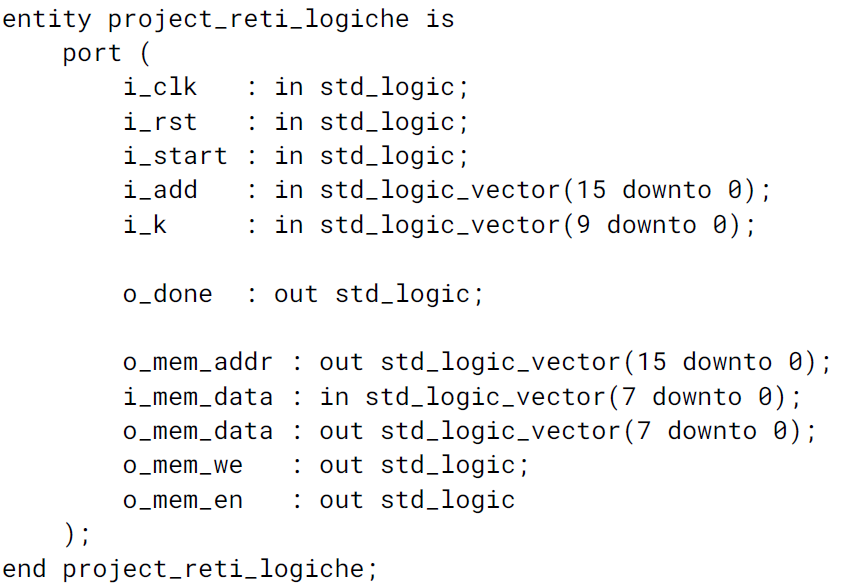
\includegraphics[width=0.5\textwidth]{specifica.png}
    \label{fig:Functional specification - Architecture interface}
\end{figure}

The system also interfaces with a byte-addressed memory with $2^{16}$ words of \(1\) Byte each.

The operations to be performed in sequence, once started, depend on the values \texttt{ADD} and \texttt{K} provided by the inputs \texttt{i\_add} and \texttt{i\_k}. Memory reading must start from address \texttt{ADD} for a total of 2K words, divided into even positions (where reading starts), which indicate significant values, and odd positions, which indicate the credibility value of the previous significant value. The system's task is to replace null significant values with the last non-null significant value read, and set its credibility value accordingly. If a non-null value is read, its credibility is set to \texttt{31}, while for each consecutive null significant value read, the credibility is decremented. If credibility reaches \texttt{0}, it remains at that value without further decrementing until the first non-null significant value is read.

If a null significant value is read at the beginning of the operation sequence, and as long as it remains so, it is left null and its credibility is also set to \texttt{0}. For subsequent operation sequences and after each reset, the operating logic remains the same.

The signals \texttt{o\_mem\_addr}, \texttt{i\_mem\_data}, \texttt{o\_mem\_data}, \texttt{o\_mem\_we}, \texttt{o\_mem\_en} are used to interface with the memory, with the obvious meanings suggested by their names, while \texttt{i\_clk} is the clock signal that synchronizes all other signals. In particular, except for the only asynchronous signal \texttt{i\_rst}, all signals are to be interpreted on the rising edge of the clock. The other signals are:

\begin{enumerate}
    \item \textbf{i\_rst}: asynchronous signal that resets the system. \texttt{i\_start} can be raised only after \texttt{i\_rst} has been lowered. The system's behavior before the first time \texttt{i\_rst} is set high is unspecified.
    \item \textbf{i\_start}: indicates the start of operations. It remains high until \texttt{o\_done} becomes '1', after which it must be lowered. After both \texttt{o\_done} and \texttt{i\_start} are lowered, another sequence of operations can be started directly using \texttt{i\_start}, without needing to reset the system again with \texttt{i\_rst}.
    \item \textbf{i\_add}: indicates the ADD value of the functional specification.
    \item \textbf{i\_k}: indicates the K value of the functional specification.
    \item \textbf{o\_done}: signals the end of the operation sequence when it becomes '1'. Once raised, there should be no further communication with the memory, and it must be lowered after \texttt{i\_start} goes to '0'.
\end{enumerate}

An example of a possible sequence of such operations is given, with ADD=10 and K=10:

\begin{table}[htbp]
    \begin{adjustwidth}{-1.cm}{}
    \centering
    \begin{tabular}{|c|c|c|c|c|c|c|c|c|c|c|c|c|c|c|c|c|c|c|c|c|c|c|}
        \hline
        Addr & 10 & 11 & 12 & 13 & 14 & 15 & 16 & 17 & 18 & 19 & 20 & 21 & 22 & 23 & 24 & 25 & 26 & 27 & 28 & 29 & 30 & 31 \\
        \hline
        Before & 0 & 0 & 128 & 0 & 64 & 0 & 0 & 0 & 0 & 0 & 100 & 0 & 1 & 0 & 0 & 0 & 1 & 0 & 23 & 0 & 0 & 0 \\
        After & 0 & 0 & 128 & 31 & 64 & 31 & 64 & 30 & 64 & 29 & 100 & 31 & 1 & 31 & 1 & 30 & 1 & 31 & 23 & 31 & 0 & 0 \\
        \hline
    \end{tabular}
    \end{adjustwidth}
\end{table}


\section{Architecture}
Below is a description of the architecture designed and implemented for the project. The signal names refer to those used in the VHDL code of the main architecture. Overall, the architecture is divided into 3 independent modules and a state machine that manages the control signals. Input/output signals directly managed by the architecture are highlighted in red, while control signals managed by the FSM (i.e., the FSM outputs) are highlighted in blue. Green signals are the reset and clock, present in the registers, while the remaining signals are internal signals (corresponding to \texttt{signal} in VHDL). The number of bits for each signal is indicated in parentheses.

The basic architectural modules used are (with reference to the name of the respective VHDL entities):
\begin{itemize}
    \item \textbf{mux}: a standard MUX with 2 inputs of 16 bits, 1 output of 16 bits, and a selection bit.
    \item \textbf{reg16}: a synchronous (flip-flop) 16-bit register, with an asynchronous reset signal and a load signal that enables writing when high.
    \item \textbf{addr16}: a 16-bit adder implemented using 16 full-adders (actually used only as an incrementer or decrementer).
\end{itemize}

\subsection{Module 1: Memory Address Manager}

\begin{figure}[htbp]
  \centering
  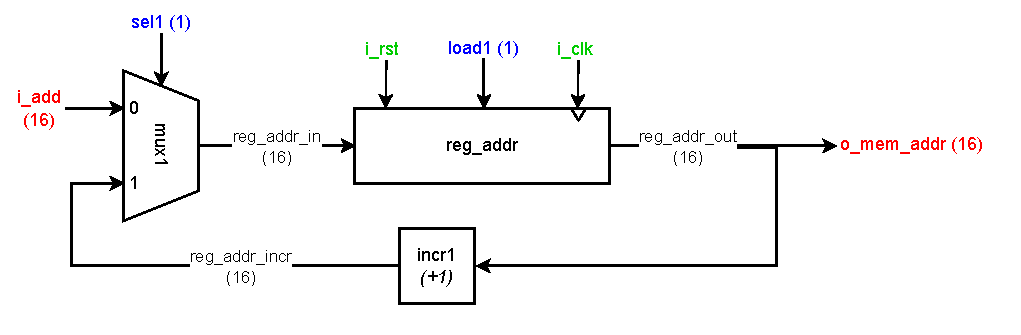
\includegraphics[width=0.8\textwidth]{modulo1.pdf}
%  \caption{Module 1: Memory Address Manager}
  \label{fig:Module 1: Memory Address Manager}
\end{figure}

The bit \texttt{\textcolor{blue}{sel1}} sends to the input of the \texttt{reg\_addr} register either the signal \texttt{\textcolor{red}{i\_add}} (for initialization) or the output of the register itself after it has been incremented (i.e., the output of the \texttt{incr1} module, which performs the +1 operation). Writing to the \texttt{reg\_addr} register is controlled by the bit \texttt{\textcolor{blue}{load1}}. The output of the register represents the \texttt{\textcolor{red}{o\_mem\_addr}} output of the entire architecture.

The VHDL implementation is fully Structural.

\subsection{Module 2: Iteration Counter Manager}

\begin{figure}[H]
  \centering
  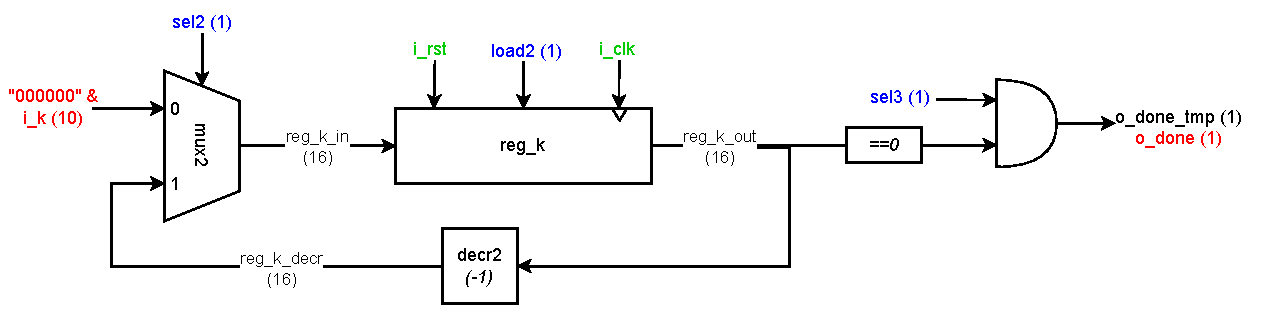
\includegraphics[width=0.82\textwidth]{modulo2.pdf}
%  \caption{Module 2: Iteration Counter Manager}
  \label{fig:Module 2: Iteration Counter Manager}
\end{figure}

The bit \texttt{\textcolor{blue}{sel2}} sends to the input of the \texttt{reg\_k} register either the signal \texttt{\textcolor{red}{i\_k}} (for initialization) or the output of the register itself after it has been decremented (i.e., the output of the \texttt{decr2} module, which performs the -1 operation). Writing to the \texttt{reg\_k} register is controlled by the bit \texttt{\textcolor{blue}{load2}}. The \texttt{==0} module outputs ‘1’ if \texttt{reg\_k\_out} is zero, ‘0’ otherwise, and, ANDed with the bit \texttt{\textcolor{blue}{sel3}}, defines the output \texttt{\textcolor{red}{o\_done}}.

The VHDL implementation is mixed, almost entirely Structural except for a Behavioural part (i.e., a \texttt{process}) to define the output \texttt{\textcolor{red}{o\_done}} as a function of \texttt{reg\_k\_out} and \texttt{\textcolor{blue}{sel3}}. The auxiliary signal \texttt{o\_done\_tmp} allows reading \texttt{\textcolor{red}{o\_done}} (as an input to the FSM), which otherwise would be only an output (not readable) of the architecture.

\subsection{Module 3: Memory Interaction Manager}

\begin{figure}[H]
  \centering
  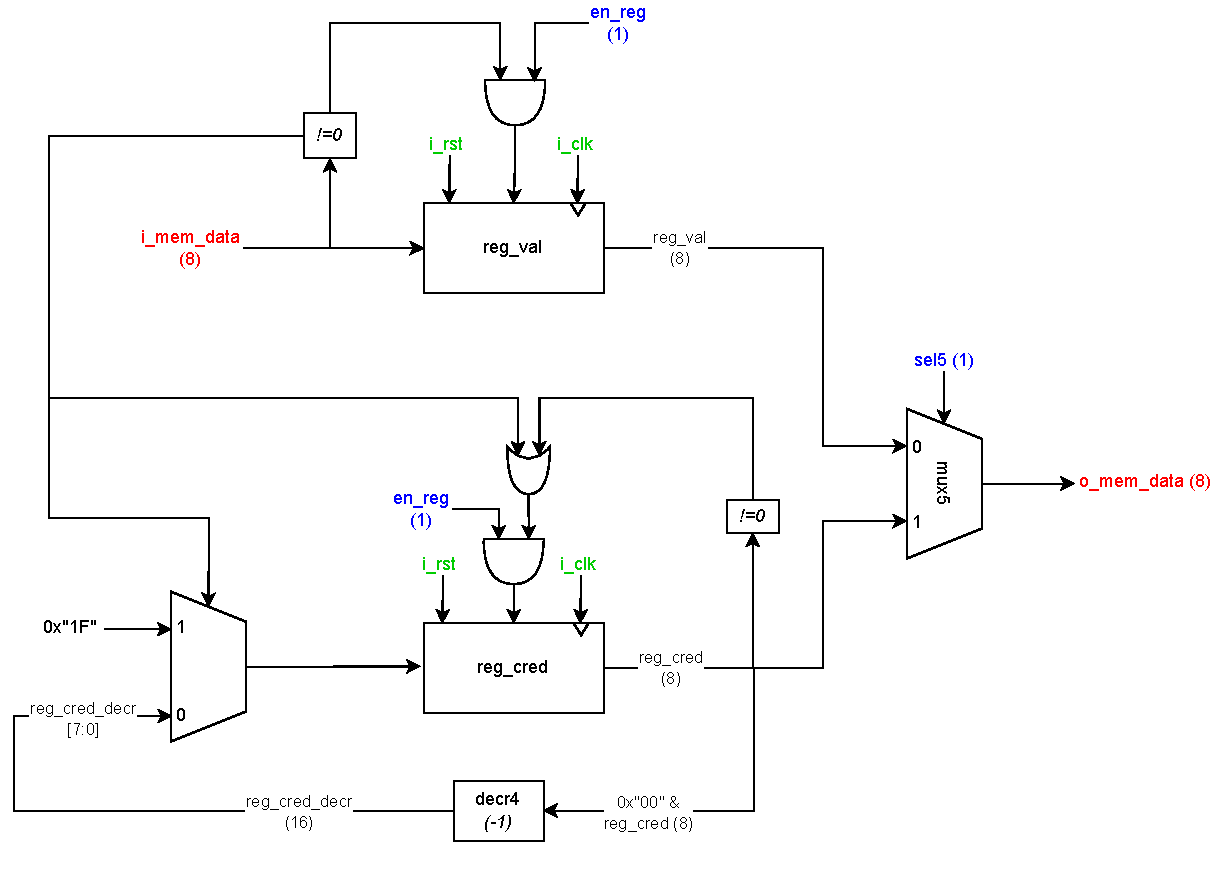
\includegraphics[width=0.95\textwidth]{modulo3.pdf}
%  \caption{Module 3: Memory Interaction Manager}
  \label{fig:Module 3: Memory Interaction Manager}
\end{figure}

Three main parts can be identified:
\begin{itemize}
    \item \textbf{reg\_val register}: register that stores the last non-zero value read. It is enabled for writing if the bit \texttt{\textcolor{blue}{en\_reg}} is high and the value \texttt{\textcolor{red}{i\_mem\_data}} is non-zero (used to store the value if it is non-zero, otherwise the last non-zero value is kept in memory).
    \item \textbf{reg\_cred register}: The input is either the value 31 (decimal) or its decremented output (i.e., the output of \texttt{decr4}, which performs the -1 operation). The choice of input depends on whether the signal \texttt{\textcolor{red}{i\_mem\_data}} is zero (if the value read is non-zero, we set 31 as the standard credibility value, otherwise we decrement the current credibility). Writing to the register occurs if \texttt{\textcolor{blue}{en\_reg}} is high and either \texttt{\textcolor{red}{i\_mem\_data}} or the current credibility value are non-zero (specifically, we must check \texttt{reg\_cred!=x"00"} to avoid further decrementing credibility when zero is reached).
    \item \textbf{mux5}: selects whether to output (\texttt{\textcolor{red}{o\_mem\_data}}) the output of the \texttt{reg\_val} register or \texttt{reg\_cred} based on the bit \texttt{\textcolor{blue}{sel5}}.
\end{itemize}

The VHDL implementation is almost completely Behavioural, except for the use of Structural style to manage only the \texttt{decr4} module.

\subsection{FSM}

\begin{figure}[H]
  \centering
  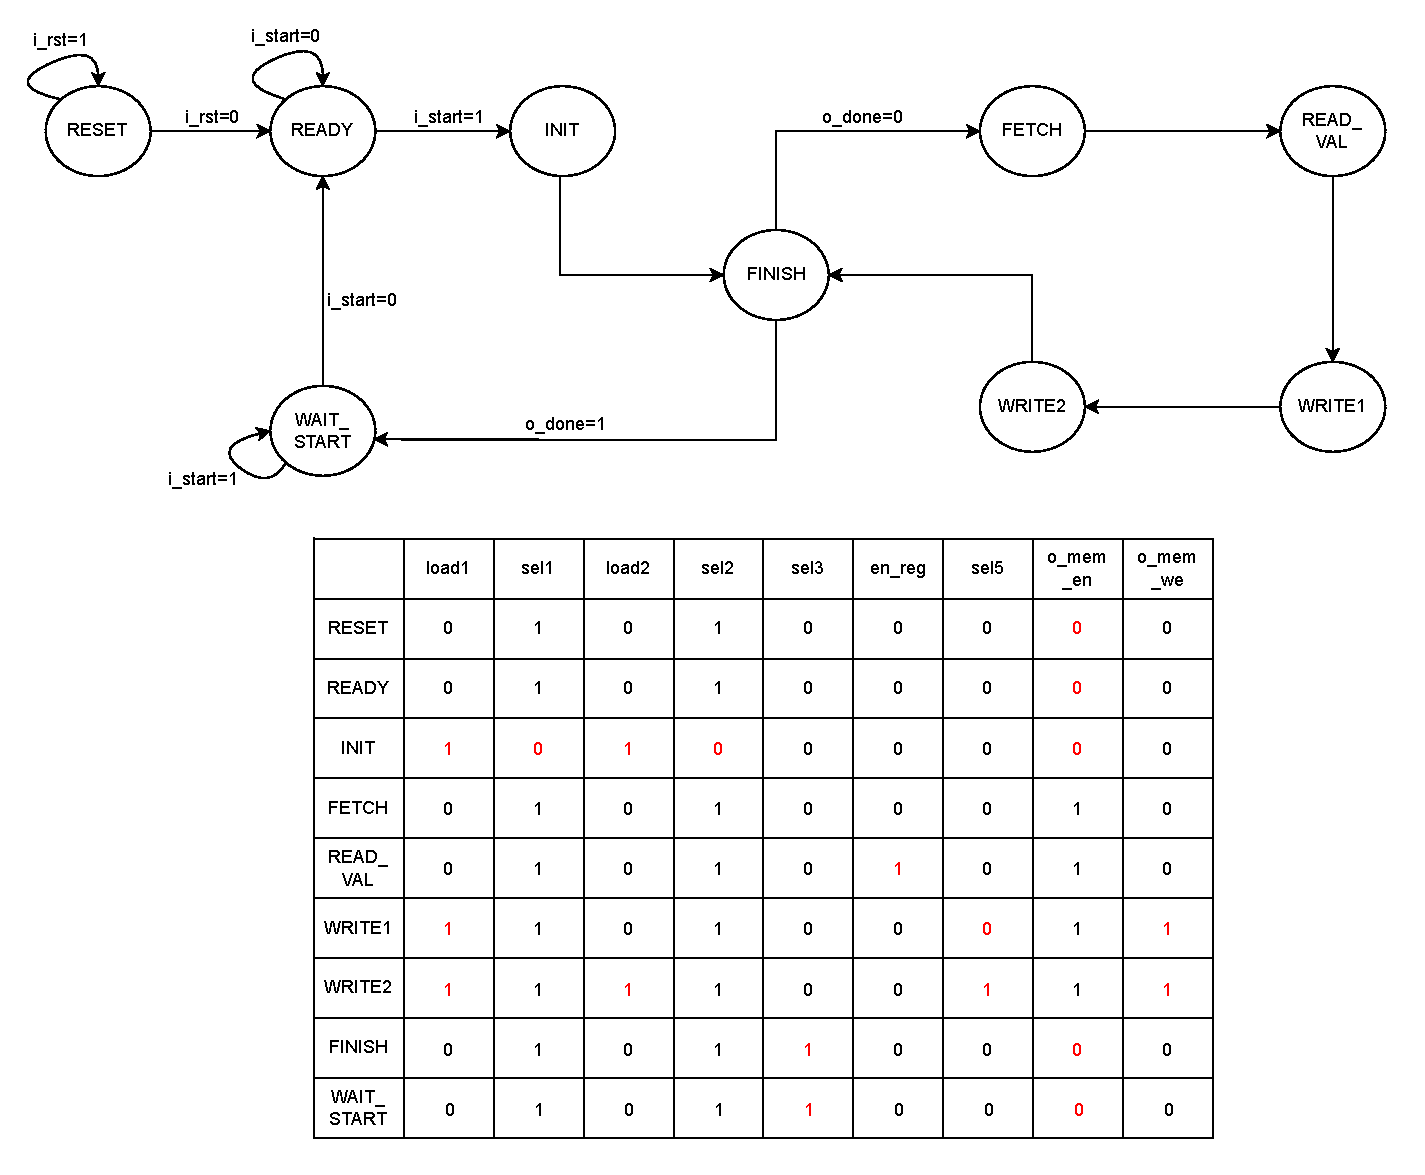
\includegraphics[width=1\textwidth, trim=0cm 11cm 0cm 0cm, clip]{modulofsm.pdf}
%  \caption{FSM}
  \label{fig:FSM}
\end{figure}

\begin{table}[htbp]
\centering
\begin{tabular}{|c|*{9}{c|}}
\hline
& load1 & sel1 & load2 & sel2 & sel3 & en\_reg& sel5 & o\_mem\_en & o\_mem\_we \\
\hline
RESET & 0 & 1 & 0 & 1 & 0 & 0 & 0 & \textcolor{red}{0} & 0 \\
\hline
READY & 0 & 1 & 0 & 1 & 0 & 0 & 0 & \textcolor{red}{0} & 0 \\
\hline
INIT & \textcolor{red}{1} & \textcolor{red}{0} & \textcolor{red}{1} & \textcolor{red}{0} & 0 & 0 & 0 & \textcolor{red}{0} & 0 \\
\hline
FETCH & 0 & 1 & 0 & 1 & 0 & 0 & 0 & 1 & 0 \\
\hline
READ\_VAL & 0 & 1 & 0 & 1 & 0 & \textcolor{red}{1} & 0 & 1 & 0 \\
\hline
WRITE1 & \textcolor{red}{1} & 1 & 0 & 1 & 0 & 0 & \textcolor{red}{0} & 1 & \textcolor{red}{1} \\
\hline
WRITE2 & \textcolor{red}{1} & 1 & \textcolor{red}{1} & 1 & 0 & 0 & \textcolor{red}{1} & 1 & \textcolor{red}{1} \\
\hline
FINISH & 0 & 1 & 0 & 1 & \textcolor{red}{1} & 0 & 0 & \textcolor{red}{0} & 0 \\
\hline
WAIT\_START & 0 & 1 & 0 & 1 & \textcolor{red}{1} & 0 & 0 & \textcolor{red}{0} & 0 \\
\hline
\end{tabular}
%\caption{Uscite della FSM}
\label{tab:Uscite della FSM}
\end{table}
The state machine manages the control signals by passing through 9 states. It was designed as a Moore machine, so the outputs can be indicated in a separate table as a function of only the current state. In the table, outputs that differ from the default (as written in the VHDL FSM code) are highlighted in red.

The states are:
\begin{table}[H]
    \centering
%    \caption{Description of FSM States}
    \begin{tabular}{|l|p{15cm}|}
%        \hline
%        \textbf{State} & \textbf{Description} \\
        \hline
        RESET & FSM reset state, where it remains until \texttt{i\_rst} goes low again \\
        \hline
        READY & Wait until \texttt{i\_start} is set high to begin the operation sequence \\
        \hline
        INIT & Set the initial values of the \texttt{reg\_addr} and \texttt{reg\_k} registers to start the operation sequence \\
        \hline
        FETCH & Enable memory reading to set \texttt{i\_mem\_data} with the significant value to be considered for this iteration \\
        \hline
        READ\_VAL & Based on \texttt{i\_mem\_data}, set the correct values for this iteration in the \texttt{reg\_val} and \texttt{reg\_cred} registers \\
        \hline
        WRITE1 & Write the value of \texttt{reg\_val} to memory. \newline Increment \texttt{reg\_addr} to prepare for writing the credibility value \\
        \hline
        WRITE2 & Write the value of \texttt{reg\_cred} to memory. \newline Increment \texttt{reg\_addr} to prepare for the next iteration \newline Decrement \texttt{reg\_k} to mark the iteration as completed \\
        \hline
        FINISH & State corresponding to the end of an iteration, where there is no communication with memory. If \texttt{i\_k} has not reached 0, start a new iteration from FETCH. Otherwise, move to WAIT\_START \\
        \hline
        WAIT\_START & Wait until \texttt{i\_start} goes low again \\
        \hline
    \end{tabular}
\end{table}

The VHDL implementation is the standard one also seen in class, with 2 separate processes to manage the next state function and the output function.
\section{Experimental Results}
\subsection{Synthesis}

The described architecture, once implemented in VHDL, can be synthesized and simulated as if it were on a real FPGA (the one used for synthesis is the suggested Artix-7 FPGA xc7a200tfbg484-1), through post-synthesis functional simulation. In particular, we can verify certain aspects based on the post-synthesis simulation of the example testbench provided for the project.

Using the TCL command \texttt{report\_utilization}, it can be observed that no latches were synthesized, as intended. Instead, 52 flip-flops are generated, which the synthesis tool likely used to manage the 16 bits of the \texttt{reg\_addr} and \texttt{reg\_k} registers, the 8 bits of the \texttt{reg\_val} and \texttt{reg\_cred} registers, and 4 bits to handle the 9 states of the FSM.

\begin{figure}[h]
    \centering
    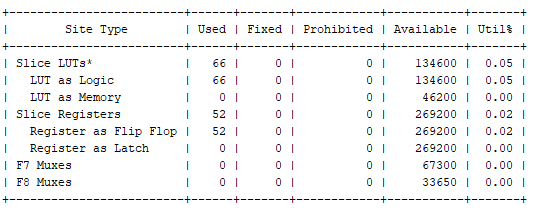
\includegraphics[width=0.5\textwidth]{report flip-flop used.png}
    %\caption{Report utilization: Number of flip-flops used}
    \label{fig:Report utilization: Number of flip-flops used}
\end{figure}

Furthermore, using the \texttt{report\_timing} command, since there is a constraint that signal delays must not exceed the clock period of 20ns, it can be seen that the slack time (the time within the clock period during which signals are stable, with no operations being performed) is largely positive (16.213 ns). Therefore, the proposed architecture does not appear to have any issues regarding signal delays.

\begin{figure}[h]
    \centering
    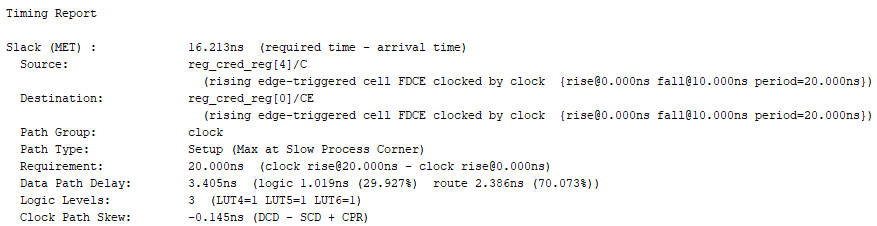
\includegraphics[width=0.8\textwidth]{report slack-time.png}
    %\caption{Report timing: Slack Time}
    \label{fig:Report timing: Slack Time}
\end{figure}

\subsection{Simulation}

\subsubsection{Testbench 1}

K = 36, ADD = 100
\begin{table}[htbp]
    \begin{adjustwidth}{-1.75cm}{}
    \centering
%    \caption{Example Table}
    \begin{tabular}{|c|*{20}{c|}}
        \hline
        Addr & 100 & 101 & 102 & 103 & 104 & 105 & 106 & 107 & 108 & 109 & 110 & 111 & 112 & 113 & 114 & 115 & 116 & 117 & 118 & 119 \\
        \hline
        Prima & 33 & 0 & 0 & 0 & 0 & 0 & 0 & 0 & 0 & 0 & 0 & 0 & 0 & 0 & 0 & 0 & 0 & 0 & 0 & 0 \\
        Dopo & 33 & 31 & 33 & 30 & 33 & 29 & 33 & 28 & 33 & 27 & 33 & 26 & 33 & 25 & 33 & 24 & 33 & 23 & 33 & 22 \\
        \hline
        Addr & 120 & 121 & 122 & 123 & 124 & 125 & 126 & 127 & 128 & 129 & 130 & 131 & 132 & 133 & 134 & 135 & 136 & 137 & 138 & 139 \\
        \hline
        Prima & 0 & 0 & 0 & 0 & 0 & 0 & 0 & 0 & 0 & 0 & 0 & 0 & 0 & 0 & 0 & 0 & 0 & 0 & 0 & 0 \\
        Dopo & 33 & 21 & 33 & 20 & 33 & 19 & 33 & 18 & 33 & 17 & 33 & 16 & 33 & 15 & 33 & 14 & 33 & 13 & 33 & 12 \\
        \hline
        Addr & 140 & 141 & 142 & 143 & 144 & 145 & 146 & 147 & 148 & 149 & 150 & 151 & 152 & 153 & 154 & 155 & 156 & 157 & 158 & 159 \\
        \hline
        Prima & 0 & 0 & 0 & 0 & 0 & 0 & 0 & 0 & 0 & 0 & 0 & 0 & 0 & 0 & 0 & 0 & 0 & 0 & 0 & 0 \\
        Dopo & 33 & 11 & 33 & 10 & 33 & 9 & 33 & 8 & 33 & 7 & 33 & 6 & 33 & 5 & 33 & 4 & 33 & 3 & 33 & 2 \\
        \hline
        Addr & 160 & 161 & 162 & 163 & 164 & 165 & 166 & 167 & 168 & 169 & 170 & 171 & & & & & & & & \\
        \hline
        Prima & 0 & 0 & 0 & 0 & 0 & 0 & 0 & 0 & 1 & 1 & 0 & 1 & & & & & & & & \\
        Dopo & 33 & 1 & 33 & 0 & 33 & 0 & 33 & 0 & 1 & 31 & 1 & 30 & & & & & & & & \\
        \hline
    \end{tabular}
    \end{adjustwidth}
\end{table}
This testbench mainly checks the correct decrement of \texttt{reg\_k}, which starts from 31 (with the first non-zero value 33 at address 100) and is decremented down to 0, where it remains for 3 iterations. It also shows that non-zero values at addresses intended for credibility do not cause any issues.
Moreover, since this is the first testbench presented, it correctly tests the general behavior, the handling of logic based on the \texttt{i\_start} and \texttt{i\_rst} signals, and the correct management of the signals \texttt{o\_done}, \texttt{o\_mem\_en}, \texttt{o\_mem\_we} (for which there are corresponding \texttt{assert} statements in the testbench).

\subsubsection{Testbench 2}

K = 7, ADD = 65522
\begin{table}[htbp]
    \begin{adjustwidth}{-1.75cm}{}
    \centering
 %   \caption{Example Table}
    \begin{tabular}{|c|*{14}{c|}}
        \hline
        Addr & 65522 & 65523 & 65524 & 65525 & 65526 & 65527 & 65528 & 65529 & 65530 & 65531 & 65532 & 65533 & 65534 & 65535 \\
        \hline
        Prima & 0 & 0 & 0 & 1 & 66 & 0 & 66 & 0 & 66 & 0 & 0 & 0 & 65 & 0 \\
        Dopo & 0 & 0 & 0 & 0 & 66 & 31 & 66 & 31 & 66 & 31 & 66 & 30 & 65 & 31 \\
        \hline
    \end{tabular}
    \end{adjustwidth}
\end{table}

This testbench checks the case where the initial significant values are null. It also covers the particular case in which multiple consecutive non-null significant values are equal (so, even if the same value appears again at the end, the credibility remains 31). Additionally, it verifies the edge case where the end of memory is reached.

\subsubsection{Testbench 3}

K = 0, ADD = 100
\begin{table}[H]
    \begin{adjustwidth}{-1.75cm}{}
    \centering
%    \caption{Example Table}
    \begin{tabular}{|c|*{20}{c|}}
        \hline
        Addr & 100 & 101 & 102 & 103 & 104 & 105 & 106 & 107 & 108 & 109 & 110 & 111 & 112 & 113 & 114 & 115 & 116 & 117 & 118 & 119 \\
        \hline
        Prima & 33 & 0 & 33 & 0 & & & & & & & & & & & & & & & & \\
        Dopo & 33 & 0 & 33 & 0 & & & & & & & & & & & & & & & & \\
        \hline
    \end{tabular}
    \end{adjustwidth}
\end{table}

This testbench checks the edge case where K=0, so there should be no iterations. (In this case, the first time the FSM reaches the FINISH state, o\_done is already high and it immediately transitions to the WAIT\_START state, without performing any iterations).

\subsubsection{Testbench 4}

ADD1 = 100, K1 = 5; ADD2 = 110, K2 = 5
\begin{table}[H]
    \begin{adjustwidth}{-1.75cm}{}
    \centering
%    \caption{Example Table}
    \begin{tabular}{|c|*{20}{c|}}
        \hline
        Addr & 100 & 101 & 102 & 103 & 104 & 105 & 106 & 107 & 108 & 109 & 110 & 111 & 112 & 113 & 114 & 115 & 116 & 117 & 118 & 119 \\
        \hline
        Prima & 255 & 1 & 52 & 0 & 11 & 0 & 92 & 0 & 22 & 0 & 2 & 0 & 0 & 0 & 12 & 0 & 39 & 0 & 31 & 0 \\
        Dopo1 & 255 & 31 & 52 & 31 & 11 & 31 & 92 & 31 & 22 & 31 & 2 & 0 & 0 & 0 & 12 & 0 & 39 & 0 & 31 & 0 \\
        Dopo2 & 255 & 31 & 52 & 31 & 11 & 31 & 92 & 31 & 22 & 31 & 2 & 31 & 2 & 30 & 12 & 31 & 39 & 31 & 31 & 31 \\
        \hline
    \end{tabular}
    \end{adjustwidth}
\end{table}

This testbench checks the correct handling of two consecutive operation sequences, without overlap of the managed memory segments. The second sequence is started without resetting the machine first.

\subsubsection{Testbench 5}

ADD1 = 100, K1 = 8; ADD2 = 104, K2 = 8
\begin{table}[H]
    \begin{adjustwidth}{-1.75cm}{}
    \centering
%    \caption{Example Table}
    \begin{tabular}{|c|*{20}{c|}}
        \hline
        Addr & 100 & 101 & 102 & 103 & 104 & 105 & 106 & 107 & 108 & 109 & 110 & 111 & 112 & 113 & 114 & 115 & 116 & 117 & 118 & 119 \\
        \hline
        Prima & 33 & 0 & 0 & 0 & 0 & 0 & 0 & 0 & 0 & 0 & 0 & 0 & 0 & 0 & 0 & 0 & 0 & 0 & 0 & 0 \\
        Dopo1 & 33 & 31 & 33 & 30 & 33 & 29 & 33 & 28 & 33 & 27 & 33 & 26 & 33 & 25 & 33 & 24 & 0 & 0 & 0 & 0 \\
        Dopo2 & 33 & 31 & 33 & 30 & 33 & 31 & 33 & 31 & 33 & 31 & 33 & 31 & 33 & 31 & 33 & 31 & 33 & 30 & 33 & 29 \\
        \hline
    \end{tabular}
    \end{adjustwidth}
\end{table}

This testbench checks the correct handling of two consecutive operation sequences, with partial overlap of the managed memory segments. The second sequence is started after resetting the machine.

\section{Conclusions}
The proposed testbenches (which are not the only ones used during the testing phase) appear to cover all relevant cases without being redundant. Given that the architecture behaves as expected both before and after synthesis, it is reasonable to assume that it has been correctly designed and implemented.

I am aware that the proposed VHDL implementation is not the easiest to write or the most straightforward to read, as it contains several Structural parts and adders that could have been left to VHDL to implement automatically. However, I intentionally wrote the implementation this way to explore VHDL as much as possible according to the methods presented in class.

\end{document}
